\documentclass{article}[11pt]

\usepackage[margin=1.in]{geometry}
\usepackage{listings}
\usepackage{color}

%\usepackage[T1]{fontenc}
\usepackage{courier}
\usepackage{authblk}
\usepackage{hyperref}
\usepackage{graphicx}
\usepackage{amsmath}

\definecolor{mygreen}{rgb}{0,0.6,0}
\definecolor{mygray}{rgb}{0.5,0.5,0.5}
\definecolor{mymauve}{rgb}{0.58,0,0.82}

\newcommand{\rrangle}{\rangle\!\rangle} \newcommand{\llangle}{\langle\!\langle}
\newcommand{\ket}[1]{\ensuremath{\left|#1\right\rangle}}
\newcommand{\bra}[1]{\ensuremath{\left\langle#1\right|}}
\newcommand{\braket}[2]{\ensuremath{\left\langle#1|#2\right\rangle}}
\newcommand{\ketbra}[2]{\ket{#1}\!\!\bra{#2}}
\newcommand{\braopket}[3]{\ensuremath{\bra{#1}#2\ket{#3}}}
\newcommand{\proj}[1]{\ketbra{#1}{#1}}
\newcommand{\sket}[1]{\ensuremath{\left|#1\right\rrangle}}
\newcommand{\sbra}[1]{\ensuremath{\left\llangle#1\right|}}
\newcommand{\sbraket}[2]{\ensuremath{\left\llangle#1|#2\right\rrangle}}
\newcommand{\sketbra}[2]{\sket{#1}\!\!\sbra{#2}}
\newcommand{\sbraopket}[3]{\ensuremath{\sbra{#1}#2\sket{#3}}}
\newcommand{\sproj}[1]{\sketbra{#1}{#1}}
\def\Id{1\!\mathrm{l}}
\newcommand{\Tr}{\mathrm{Tr}}
\newcommand{\cH}{\mathcal{H}}
\newcommand{\cM}{\mathcal{M}}

\lstset{ %
  backgroundcolor=\color{white},   % choose the background color; you must add \usepackage{color} or \usepackage{xcolor}
  basicstyle=\small\bf\ttfamily, % the size of the fonts that are used for the code
  breakatwhitespace=false,         % sets if automatic breaks should only happen at whitespace
  breaklines=true,                 % sets automatic line breaking
  captionpos=b,                    % sets the caption-position to bottom
  commentstyle=\color{mygreen},    % comment style
  deletekeywords={...},            % if you want to delete keywords from the given language
  escapeinside={\%*}{*)},          % if you want to add LaTeX within your code
  extendedchars=true,              % lets you use non-ASCII characters; for 8-bits encodings only, does not work with UTF-8
  frame=single,                    % adds a frame around the code
  keepspaces=true,                 % keeps spaces in text, useful for keeping indentation of code (possibly needs columns=flexible)
  keywordstyle=\color{blue},       % keyword style
  language=bash,                   % the language of the code
  morekeywords={*,...},            % if you want to add more keywords to the set
  numbers=left,                    % where to put the line-numbers; possible values are (none, left, right)
  numbersep=5pt,                   % how far the line-numbers are from the code
  numberstyle=\tiny\color{mygray}, % the style that is used for the line-numbers
  rulecolor=\color{black},         % if not set, the frame-color may be changed on line-breaks within not-black text (e.g. comments (green here))
  showspaces=false,                % show spaces everywhere adding particular underscores; it overrides 'showstringspaces'
  showstringspaces=false,          % underline spaces within strings only
  showtabs=false,                  % show tabs within strings adding particular underscores
  stepnumber=1,                    % the step between two line-numbers. If it's 1, each line will be numbered
  stringstyle=\color{mymauve},     % string literal style
  tabsize=2,                       % sets default tabsize to 2 spaces
  title=\lstname                   % show the filename of files included with \lstinputlisting; also try caption instead of title
}

\title{GST Quick Start Guide (v0.8)}
\date{\today}
\author[1]{Robin Blume-Kohout}
\author[1]{John K. Gamble}
\author[1]{Erik Nielsen}
\author[1]{Kenneth Rudinger}
\affil[1]{Sandia National Laboratories}

\renewcommand\Authands{ and }

\begin{document}
\maketitle
\tableofcontents

\newpage
\section{Executive summary}

Gate-set tomography (GST) is a method for characterizing quantum operations on as-built qubits.  If you are trying to develop a qubit, and your goal is to implement a set of quantum logic gates, and you want to find out exactly what [imperfect] transformations you're actually doing\ldots then GST is for you.

%\subsection{How GST works}

GST comprises: (i) a specification of what experiments (gate sequences) to perform; (ii) algorithms for analyzing the data to estimate the gates; and (iii) algorithms to perform meta-analysis on the estimate, providing rich debugging information about the system's operation.  Here, we summarize how the analysis works, in order to explain why we ask you to do certain experiments.

For the purposes of GST, your quantum system (typically one or more qubits) is modeled as a black box, over which you have limited control, and whose behavior can be described fully by: (1) an initial state $\rho$; (2) a measurement $\mathcal{M} = \{E_j\}$ described by its outcomes (``effects'') $E_j$; and (3) some gates (quantum operations) $\{G_k\}$.  For a single qubit, the measurement typically has just two outcomes ($\cM = \{E,\Id-E\}$), and we describe it by a \emph{single} operator $E$.

The analysis proceeds in two phases, each implemented by a different algorithm.  \emph{Linear GST} (LGST) analyzes data from certain short gate sequences (see below) using linear algebra. It is very reliable, but not very \emph{precise} (precision is comparable to standard process tomography).  \emph{Extended linear GST} (eLGST) takes this initial estimate and refines it iteratively, by incorporating data from successively longer sequences.  We implement eLGST by using an iterative least-squares algorithm (LSGST) to find a minimum-$\chi^2$ estimate to the data.

The gate sequences for LGST are based on a small set of short \emph{fiducial sequences}, denoted $\{F_i\}$.  For GST on a $d$-dimensional Hilbert space, there are $O(d^2)$ fiducials.  The role of these short gate sequences is to transform the fixed $\rho$ and $E$ into informationally complete \emph{sets} $\{\rho_i\}$ and $\{E_i\}$.  Here is a common example:
\begin{itemize}
\item The target prep/measurement are $\rho = \proj{0}$ and $E = \proj{1}$.
\item The target gates are $\pi/2$ rotations: $G_x = e^{-i(\pi/4)X}$, $G_y = e^{-i(\pi/4)Y}$.
\item We choose four fiducial sequences: $F_1 = \{\}$, $F_2 = G_x$, $F_3 = G_y$, $F_4 = G_xG_x$.
\end{itemize}
Note that the first fiducial sequence is the null sequence -- ``do nothing for no time'' -- and we denote this uniquely by ``$\{\}$''.  If the target gates are [approximately] correct, then these fiducials will map $\rho$ and $E$ to sets of states and measurements (respectively) that are informationally complete.  If the actual gates are wildly different from the targets, then these fiducials may not work well -- but LGST can detect this.

The actual gate sequences required by both phases of GST are all of the form
\begin{equation}
F_i\ S\ F_j,
\end{equation}
where $S$ denotes some sequence of gates, and $i$ and $j$ run over all fiducials.  The sequences used by LGST are all of the form $F_i\{\}F_j$ or $F_iG_kF_j$, where $G_k$ is a single gate.  LGST \emph{also} requires a few additional sequences including the null sequence $\{\}$ and single-fiducial sequences $F_i$.

The second phase of GST requires longer sequences of the form
\begin{equation}
F_i\ (J_k)^L\ F_j
\end{equation}
where the $J_k$ are short sequences called \emph{germs}, $(J_k)^L$ denotes $L$ repetitions of $J_k$, and $L$ is an integer that usually runs over $L=1,2,4,8,16,\ldots,L_{\mathrm{max}}$.  The sequences of the form $(J_k)^L$ are called \emph{germ powers}, and their role is to provide extremely high accuracy.  

Germs are chosen (in a way that is specific to the gateset) so as to ensure that every possible small variation in the $G_k$ is \emph{amplified} -- made to grow proportional to $L$ -- by one germ or another.  Designing germs to satisfy this criterion is a bit of a black art, but we can do it for your qubit.  Generally, we can design good germ sets based on the target gates.  If the target gates are sufficiently incorrect, then we may need to choose new germs based on the results from a first round of GST.

\clearpage

\section{Introduction to GST}

\subsection{What we need to know}

If you're still reading, you probably want to do GST.  In the rest of this document, you'll find essential information about how GST works, what experiments you should do, and how to record and format your data.  What you will \emph{not} find -- at least now -- is instructions on how to run the GST analysis software!  That's because we (the GST theory team) are still developing our code, and it isn't ready for release.  However, we'll be happy to analyze your data and send you the complete results, or let you run our code directly on your data through our website (see section \ref{secWebsite} below).

Setting up such a collaboration is pretty easy.  We'll need some basic initial information right off the bat, though.  This information will allow us to tell you what \emph{specific} experiments to do.  GST itself is agnostic to the nature of your qubit, but getting the best accuracy and efficiency requires some adaptation, which we prefer to do up front.
\begin{enumerate}
\item \textbf{What are your native target gates?}  In other words, what operations are you \emph{trying} to do?  Generally, labs with a working qubit have a few operations pretty well tuned up, and any other unitary (or at least any Clifford operation) can be built from those native gates.  Unlike randomized benchmarking, we aren't interested in performing general Clifford gates -- just tell us what your basic native gate set is, and we'll work with that.  
\item \textbf{In what state do you try to initialize?}
\item \textbf{What measurement do you try to do?}  If it has two outcomes (the usual situation), what is the projector or POVM effect that you call ``1'' or ``yes'' or ``success''?
\item \textbf{Roughly what is your decoherence rate?}  This is the smaller of $T_1$ and $T_2$, divided by the time required to do a gate.  We want to know many consecutive gates (chosen at random) you could do before your polarization drops by a factor of, say, $1/2$.
\item \textbf{Is there any special weirdness to your system} that differentiates it from a standard slightly-noisy qubit?
\end{enumerate}

After you've told us those things, read the rest of this document.  It will explain the basic principles and mechanics of GST.  By then, we should be ready to send you the specific information/instructions that you need to proceed.  The most important thing we'll send you is a \textbf{template dataset file}, which is a text file that lists the experiments required by GST and contains placeholders for the experimental values you'll measure (we'll explain the precise format in more detail below).  In addition to the template dataset file, we may send you two additional files that list the fiducial sequences and germ sequences, respectively. These files can aid in understanding how the set of experiments in the dataset template file were obtained, but are optional since all of the experiments you need to perform are given in the template dataset.


\subsection{What GST does and requires}\label{whatGSTDoes}

GST's main progenitors and competitors are (i) quantum process tomography and (ii) randomized benchmarking (RB).  Compared with process tomography, GST is far more robust to miscalibration, and achieves much higher accuracy.  Compared with RB, GST provides far more complete information about the experimental gates' deviation from the targets, is much more sensitive to coherent and drift errors, and does not require approximate Clifford gates.

GST models your quantum system (typically one or more qubits) as a black box.  You must have the ability to do three basic things:
\begin{enumerate}
\item Begin an experiment by initializing the qubit[s] in some repeatable state $\rho$.  GST does not assume that you know this state, or that it has any particular form.  (It should not be the maximally mixed state).
\item Apply, on demand, one of several ``gates'' -- i.e., quantum operations -- that we denote $\{G_1,G_2,\ldots G_K\}$.  GST does not assume that you know these operations, or that they have any particular form.  (They \emph{do} need to be repeatable.  And it's best if these operations are reasonably close to unitary).
\item Perform a measurement (denoted $\cM = \{E_m\}$) with 2 or more possible outcomes, and record the result.  For example, if you are measuring $\sigma_z$, and observing the state $\ket{0}$ corresponds to a ``yes'' measurement, then $E_0=\left(
\begin{array}{cc}
1 & 0 \\
0 & 0 \\
\end{array}\right)$, and 
$E_1=\left(
\begin{array}{cc}
0 & 0 \\
0 & 1 \\
\end{array}\right)$.
GST does not assume that you know this measurement, that it has any particular form, or anything about the post-measurement state.  Two outcomes are generally sufficient.  If you do not have single-shot measurements (i.e., your outputs are ensemble measurements, integrated currents, or something else that lumps together many repetitions of the same experiment), GST still works fine.  It helps if you can quantify how many ``shots'' were averaged over for a given observation.
\end{enumerate}

GST is remarkably free of assumptions -- it doesn't assume that you have particularly precise control, or low decoherence, or can do pretty good Clifford gates, or anything like that.  But it does rely on one very important assumption:  \textbf{we assume that you can perform repeatable gate operations}.  This is more or less necessary -- if you have a button labeled ``Hadamard'', but it malfunctions in some horrible systematic/periodic way (e.g., every other time you push it, it actually does a phase gate!), then all bets are off.  Random fluctuations are fine -- that's just decoherence.  But they have to be \emph{i.i.d.} fluctuations.  Systematic fluctuations over time (drift) are a problem.

All such pathological fluctuations, plus memory effects, heating, etc, can be lumped together as \emph{non-Markovian noise}.  GST assumes that each gate can be modeled by a single time-invariant, completely positive, trace-preserving (CPTP) linear map.  Anything that violates this model will be a problem.  (Note that non-Markovian noise is an equally big problem for RB, and GST is better at detecting it.)

That said, the evidence suggests that almost \emph{every} qubit system has some non-Markovian behavior.  GST incorporates some fairly powerful routines for detecting non-Markovian effects, and we can even provide extensive debugging information about it, to help you eliminate it.  But all of this information is essentially of the form ``the Markovian model failed'' -- we do not (and cannot) provide a full characterization of non-Markovian noise, and it is even possible (in principle) that certain pernicious forms of non-Markovian noise might go completely undetected.  However, to the extent that we can detect non-Markovian noise, we can determine at what time in your experiment it becomes relevant, and on what gates it appears.

\subsection{GST outputs and inputs}

The \emph{output} of GST is a simultaneous estimate of: (i) the state $\rho$ in which you are initializing; (ii) each of the gates $G_k$ (for $k=1\ldots K$) that you can implement; and (iii) the ``effects'' $\{E_m\}$ that describe your measurement.  Most single-qubit experiments involve a measurement with just two outcomes, so the measurement is $\cM = \{E,\Id-E\}$.  In this document, we assume this form for convenience and just represent the measurement by a single effect $E$.  But if your measurement has more than 2 outcomes, rest assured GST can deal with it.

The usual way to represent $\rho$ and $E$ is as $d\times d$ positive operators on a $d$-dimensional Hilbert space (e.g., $d=2$ for a single qubit).  But be aware that Hilbert space dimension is \emph{not} as objective as we might wish -- most ``qubit'' systems have much larger Hilbert spaces available to them, and it is only by your hard work that your system \emph{behaves} like a $d$-dimensional qudit.  In the future, GST will tell \emph{you} what $d$ appears to be for your system.  Currently, you specify $d$, and GST tells you whether the data are consistent with it.

Instead of representing $\rho$ and $E$ as $d\times d$ matrices, GST represents them as $d^2$-dimensional vectors, in the vector space of Hermitian matrices, e.g.
\begin{equation}
\rho = \frac{1}{2} \left(\begin{array}{cc}1+n_z&n_x-in_y\\ n_x+in_y&1-n_z\end{array}\right) \longrightarrow \sket{\rho} = \frac{1}{\sqrt{2}}\left(\begin{array}{c}1\\ n_x \\ n_y\\ n_z\end{array}\right).
\end{equation}
We normally use the orthonormal basis defined by the (normalized) Pauli operators.  $E$ is a row vector, and the inner product between $\rho$ and $E$ is a probability (Born's Rule) that we call the \emph{SPAM parameter}
\begin{equation}
\mathrm{Pr_{SPAM}} = \sbraket{E}{\rho} = \Tr[E\rho].
\end{equation}
Gates ($G_k$) are represented by $d^2\times d^2$ matrices, which transform states (i.e., $\sket{\rho} \to G_k\sket{\rho}$).  (Note: these are \emph{not} Choi or $\chi$ matrices.  Those do not combine by multiplication!  The $G_k$ are linear operators on the space of states, sometimes referred to as ``Liouville'' superoperators.) Experiments are therefore represented by \emph{gate sequences} of the form
\begin{equation*}
S = G_{s_1}G_{s_2}\ldots G_{s_{L-1}}G_{s_L}.  
\end{equation*}
\textbf{Whenever we talk about a gate string or gate sequence, the first gate to be applied appears on the left}, and so you can read the sequence $S$ as ``do $G_{s_1}$, then $G_{s_2}$, etc., etc., until you do $G_{s_L}$ last''.  Be aware of the potential for confusion when writing down the mathematical expression for the measurement probability associated to $S$:
\begin{equation}
\mathrm{Pr_S(E|\rho)} = \sbraopket{E}{G_{s_L}G_{s_{L-1}}\ldots G_{s_2}G_{s_1}}{\rho}.
\end{equation}
In this expression $G_{s_1}$ appears on the right, since that matrix transforms $\sket{\rho}$ first.

To do GST, you must implement a list of specific gate sequences (usually between 50 and a few thousand).  Each must be repeated many ($N$) times to obtain an estimate of the probability in the previous equation.  The data \emph{input} to GST comprises a list of these observed counts (or their ensemble averages).

\subsection{The gauge}

Standard tomography reports an unambiguous and unique estimate of the state or process.  But this comes at the cost of absolute dependence on an unrealistic assumption:  that you can (1) prepare absolutely reliable and precalibrated states like $\ket{0}$ and $\ket{+}$, and (2) perform several perfectly calibrated measurements of (e.g.) $\sigma_x$, $\sigma_z$, etc.  GST makes no such demands.  The price is a \emph{gauge} freedom in the results.  If the gate set $\{\sket{\rho},\sbra{E},\{G_k\}\}$ is a good fit, then so is the (apparently distinct) gateset given by
\begin{equation}
\{\mathbf{T}\sket{\rho},\sbra{E}\mathbf{T}^{-1},\{\mathbf{T}G_k\mathbf{T}^{-1}\}\},
\end{equation}
for any invertible $d^2\times d^2$ matrix $\mathbf{T}$.  Such transformations have no observable effect, as $\sbra{E} \mathbf{T}^{-1} \left(\mathbf{T} G_k \mathbf{T}^{-1}\right) \mathbf{T} \sket{\rho} = \sbra{E} G_k \sket{\rho}$.  $\mathbf{T}$ can be a change of basis, or a non-unitary (and non-trivial) gauge transformation.

GST typically finds an estimate in an \emph{arbitrary} gauge.  This raw estimate might look very different from what you had in mind -- even if it represents exactly the gates you were trying to implement!  GST gets around this problem by \emph{gauge optimization}.  This means searching for a gauge that makes the estimated gates as close as possible to your \emph{target} gates.  For this reason, GST needs to have the target (goal) gates specified in advance.  They are used \emph{only} to optimize the gauge, and the resulting gauge transformations have no physical impact whatsoever, so there is no possibility of ``cheating'' (a.k.a. self-fulfilling prophecy).

Be aware that:
\begin{enumerate}
\item Gauge transformations do not respect the trace-preserving (TP) or complete positivity (CP) properties of quantum processes.
\item The GST software [currently] chooses a gauge in which the estimates are as close as possible to your targets, \emph{not} one in which they are as close as possible to CPTP.
\end{enumerate}
Therefore, if you see violations of CP or TP that are comparable in magnitude to the difference between the estimated gates and your targets, \textbf{these may be artifacts of the gauge optimization process}.

\subsection{Buffer errors and clock cycles} \label{bufferErrors}

In Sec.~\ref{whatGSTDoes}, we briefly discussed the concept of non-Markovian noise, and how it is detrimental to GST.
One of the types of non-Markovian noise that is preventable in most experimental setups is called a \emph{buffer error}.
A buffer error occurs whenever whatever pulse is generating a gate alters a subsequent gate.
Hence, when applying a gate, it is important to ``buffer" in time whatever active control is being used to implement the gate. 
The reason for this is to ensure that each gate is a module that does not depend on the gates that precede it, since such a dependence would amount to non-Markovian noise.

In order to ensure that buffer errors do not occur, we suggest that GST experiments impose a clock cycle, where gates take place at some regular rate. The clock should be chosen such that the elementary gates are sufficiently spread out to avoid buffer errors. 
Note that if two gates take different amounts of time to implement, it is perfectly acceptable to have one gate occupy multiple clock counts. 
Imposing a clock rate also gives a natural notion of an idle gate, which we can use GST to characterize, and will be important for considering realistic quantum circuits.

\section{Input data formats: What GST needs to run}

GST is implemented by a collection of Python functions.  It reads data from columnar-data ASCII text files.  The formats are intended to be both human- and machine-readable.  There are three different input file formats, each for storing a different type of data.
\begin{itemize}
\item a \textbf{data file}, which contains a list of gate sequences and corresponding experimental counts.  This is the file you need to generate which contains your experimental data, making this is the most important file format to understand.  To make generating data files as painless as possible, we'll send you a template data file which is a valid-format data file but contains zeros instead of actual data.
\item a \textbf{gate sequence file}, which contains a list of gate sequences (typically fiducial gate sequences or germ gate sequences).  This is essentially the same format at the data file without columns containing data counts.
\item a \textbf{gateset file}, which describes a the gates, state prep, and measurements which together comprise a ``gate set''.  This format is typically used to specify your ``target gateset'', that is, the gate set you were trying to perform.
\end{itemize}

\noindent If you want to know more details about the different file formats, please read the rest of this section.  If the template data set file you've received is intuitive enough and you want to just replace the zeros there with your data then you can skip to section \ref{secNextSteps}.

\subsection{Data file format}
GST input data is given as a list of gate sequences associated with measurement counts.  This is done via a text file containing three space-delimited columns:
\begin{itemize}
\item a gate string ($s$)
\item the number of ``up'' counts ($n_s$) %or frequencies ($f_s$)
\item the total number of times ($N_s$) that $s$ was performed.
\end{itemize}
If you don't have single-shot measurements (e.g., you measure an ensemble or integrated current), then give us your best estimate of $N_s$, and report $n_s = f_sN_s$, where $f_s$ is your observed fraction (a floating point value between 0 and 1).

A ``gate string'' specifies the sequence of gates performed.  It is simply a list of gate names concatenated together.  In this document, we typically denote gates as $G_k$, but in the data file, a valid gate name is any string of the form ``\texttt{G****}'' where any lower-case alphanumeric string can follow ``\texttt{G}''.  Valid gatenames include ``\texttt{G1}'', ``\texttt{Gx}'', ``\texttt{Gx2}'', ``\texttt{Gfoobar}'', and ``\texttt{G1foo2bar}''.  Note that capital letters are considered ``reserved'', and cannot be used following the initial ``G'', e.g. ``\texttt{GI}'' is not an acceptable name, but ``\texttt{Gi}'' is.  There's one special case:  the empty or null gate sequence is denoted by ``\texttt{\{\}}''.

For example, suppose you have three gates and you denote them by G1, G2 and G3.  A GST input file could look like this:
% (note that blank lines are ok, the \# sign can be used for comments, but ``\#\#'' indicates a mandatory header line):

\begin{minipage}{\linewidth}
\begin{lstlisting}[frame=single,caption=Example data file]
#My Experimental data
## Columns = plus count, count total
{}            10  100
G1G2          98  100
G2G3          0   100
G1G3G3G2      23  100
\end{lstlisting}
\end{minipage}

Some important points about this format:
\begin{enumerate}
\item Blank lines are okay, and will be ignored by the parser.
\item Lines beginning with a single \# are comments, and will be ignored.
\item However, \#\# indicates a [mandatory] header line (the parser will crash if it's not there)!  %If you are reporting \emph{frequencies} (between $0$ and $1$) rather than \emph{counts}, change ``plus count'' to ``plus frequency''.
\end{enumerate}

Long sequences can get very unwieldy.  For this reason, the data file specification also includes a simple notation for repeated sequences:  ``\texttt{Gx\string^{}4}'' equates to ``\texttt{GxGxGxGx}''.  Parentheses are used to repeat sequences:  ``\texttt{(G1G2)\^{}3}'' equates to ``\texttt{G1G2G1G2G1G2}''.  This notation may be mixed freely with the standard notation, e.g. ``\texttt{Gx(G1G2)\^{}2(Gy)\^{}3}'' equates to ``\texttt{GxG1G2G1G2GyGyGy}''.

\subsection{Gate sequences file format}
Most of the the gate sequences contained in the data file will have the form $F_i$ \texttt{(}$J_k$\texttt{)\^{}}$L$ $F_j$, where $J_k$ is a germ gate sequence, $F_i$ and $F_j$ are fiducial gate sequences, and $L$ is an integer (e.g.~\texttt{Gx(Gy)\^{}4Gx} or \texttt{GxGy(GyGx)\^{}2Gx}).  Internally, GST needs to know the sets of fiducial gate sequences and of germ gate sequences that you are using.  Lists of gate sequences are stored in GST's gate sequence file format, which specifies a single gate string per line using the same gate-string-format as a data file (see above).  For example, the four fiducial sequences $\{\}$, $G_1$, $G_2$, and $G_1G_1$ would be stored in a file like this (usually named something like \texttt{fiducials.txt}):

\begin{minipage}{\linewidth}
\begin{lstlisting}[frame=single,caption=Example fiducial list]
#My Fiducials
{}
G1
G2
G1G1
\end{lstlisting}
\end{minipage}

\noindent The germ gate sequences are stored in a file with exactly the same format (usually named something like \texttt{germs.txt}).

\subsection{Gateset file format}
It's also useful to store state preparation, gates, and measurement information, which we lump together into an object called a ``gate set''.  The gateset file format does this very thing.  It contains several blank-line-delimited blocks.  The first line of each block labels that block, the second line specifies the format of the block, and the remaining lines contain the values (in the specified format).  There is one block for each state preparation, gate, or measurement.  The state preparation should be labeled ``\texttt{rho}'', the measurement ``\texttt{E}'', and the gates by their gate names as discussed above.  Using the ``\texttt{StateVec}'' and ``\texttt{UnitaryMx}'' formats, preparation and measurement operationts are given as vectors in Hilbert space, and target gates are given by unitary matrices describing how the gate acts on pure states, respectively.  It is possible to specify preparations and measurements as arbitrary density matrices, and gates as arbitrary CPTP maps, but we do not cover these alternate formats here.  The example below specifies preparation in the $|0\rangle$ state and measurement in the $|1\rangle$ state, and two gates: a $\pi$ X-rotation and a $\pi/2$ X-rotation.  Gateset files are typically used to store the target gateset, that is, the preparation, gates, and measurement that you're trying to perform.

\begin{minipage}{\linewidth}
\begin{lstlisting}[frame=single,caption=Example gate set file]
# My gateset

rho
StateVec
1 0

E
StateVec
0 1

G1
UnitaryMx
0 1
1 0

G2
UnitaryMx
 1/sqrt(2)   -1j/sqrt(2)
-1j/sqrt(2)   1/sqrt(2)
\end{lstlisting}
\end{minipage}


\noindent \textbf{That's it!}  With a data file, fiducial- and germ-sequence files, and a target gateset file GST is able to generate estimates for your state preparation, measurement, and gates.  We usually create the gate sequence and target gateset files for you, so you probably only need to know how to \emph{read} the gate sequence and gate set formats, and fill in the template data set file.


\section{Next steps\label{secNextSteps}}

If you've read this far, \textbf{congratulations!}  That's about it.  The next step is for the GST theory team to identify fiducial and germ sequences that will work well for your gateset.  We'll then send you the complete set of gate sequences (probably between 100 and 5000 of them) in a template data file.  It will have placeholders (zeros) for all of the observed counts; you just need to do all those experiments (repeat each one $N$ times, where $N$ is an integer between 50 and 5000 that the theory team will suggest), and fill in the ``up'' counts and total \#-of-counts columns in the file.  Then you either email the data file back to us for analysis, or upload the file to the GST website for a similar analysis (see section \ref{secWebsite}).


\section{Cautionary tales}

We'd like to conclude with a few suggestions for things \emph{not} to do.  Worst practices, if you will.  These are some ideas that you might be tempted to implement, but really shouldn't.  We expect that this list will grow over time\ldots
\begin{enumerate}
\item \textbf{Don't combine multiple consecutive gates into a single pulse!}  It's tempting to believe that two $X$ gates can be implemented by just leaving the Hamiltonian on for twice as long. This results in large buffer errors (Sec.~\ref{bufferErrors}), which make it difficult for GST to give accurate results.
%Problem is, the operation implemented by a single ``X'' pulse depends on the rise/fall of the pulse too!  If you just extend it twice as long, you don't get $G_x^2$.  You get something [slightly or massively] different.  And this shows up as a [nasty] non-Markovian effect.  Please try to make sure that your control pulses are buffered -- ensure that they don't overlap, and don't try to compile multiple consecutive gates into a single pulse or pulse sequence.
\item \textbf{Identity is different from ``no operation'' (NOP).}  This is pretty simple:  please just be aware that there's a difference between an idle gate (i.e., you try to keep the qubit still for a microsecond) and ``nothing for no time''.  By all means, define and use an idle gate $G_i$, whose target is the $\Id$ matrix.  But don't use it in place of the NOP $\{\}$ operation (e.g., as a fiducial).
\item \textbf{Don't confuse us with composite/compiled gates.}  We are trying to characterize your \emph{native} gates.  This isn't randomized benchmarking -- we don't care about Cliffords.  If you can do a nice $\pi/2$ $Z$ rotation\ldots but you do it by chaining together three or four $X$ and $Y$ rotations\ldots it's not relevant!  Your native gates are $X$ and $Y$ rotations; don't confuse matters with extra operations that are built out of native gates.
\item \textbf{Do treat DCG sequences as ``atomic'' gates.}  If your gates are dynamically corrected (DCG), that's great.  For example, you might implement an ``idle'' gate by doing two carefully timed $X_\pi$ flips.  For GST purposes, this is a single $G_i$ operation -- we don't care about what pulses went into the operation.
\item \textbf{Do interleave the sequences!}  GST solves 99 problems, but \emph{drift} isn't one of them.  GST assumes that a ``\texttt{G1}'' operation is always the same operation, and if your operations drift slowly and systematically over time, that assumption is violated.  In order to minimize the resulting pathology (and help GST catch such behavior), we \emph{strongly} recommend that you interleave experiments instead of batching them.  That is, if you need to do $N=100$ repetitions of $500$ different sequences, do one count of each experiment.  Then go back and do another count of each experiment, etc.  Don't repeat sequence \#1 $N$ times, then repeat sequence \#2 $N$ times, etc.
\end{enumerate}


\section{The GST Website\label{secWebsite}}

In order to facilitate the rapid analysis of GST data files, we've recently created a website where you can upload your dataset files and receive a standard GST analysis of the data immediately.  Once an account has been created for you (as part of the initial collaboration phase, if you'd like), navigate to \texttt{\href{https://prod.sandia.gov/gst}{https://prod.sandia.gov/gst}} where you'll need to login with the username (the email address of someone on your group) and password we give to you.  This will bring you to the home page (Fig.~\ref{figHomePage}), where the only thing you can do is click on the ``get started'' link, so do that.  This brings you to the start page, (Fig.~\ref{figStartPage}) where you:


\begin{figure}[h!]
\begin{center}
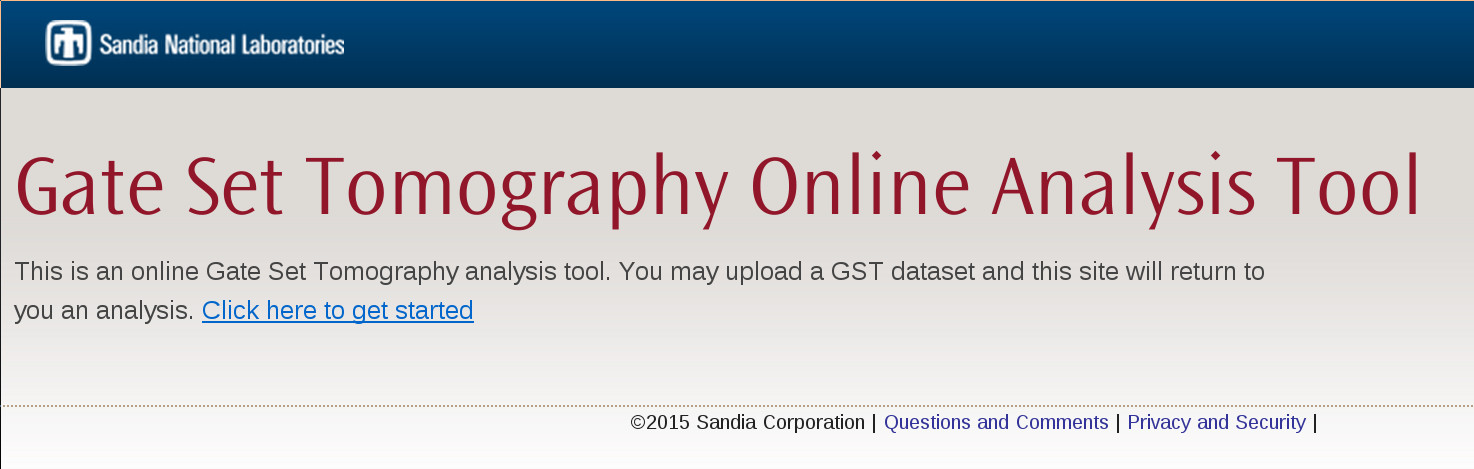
\includegraphics[width=6in]{QuickStartResources/HomePage.jpg}
\caption{GST Website Home Page\label{figHomePage}}
\end{center}
\end{figure}

\begin{figure}[h!]
\begin{center}
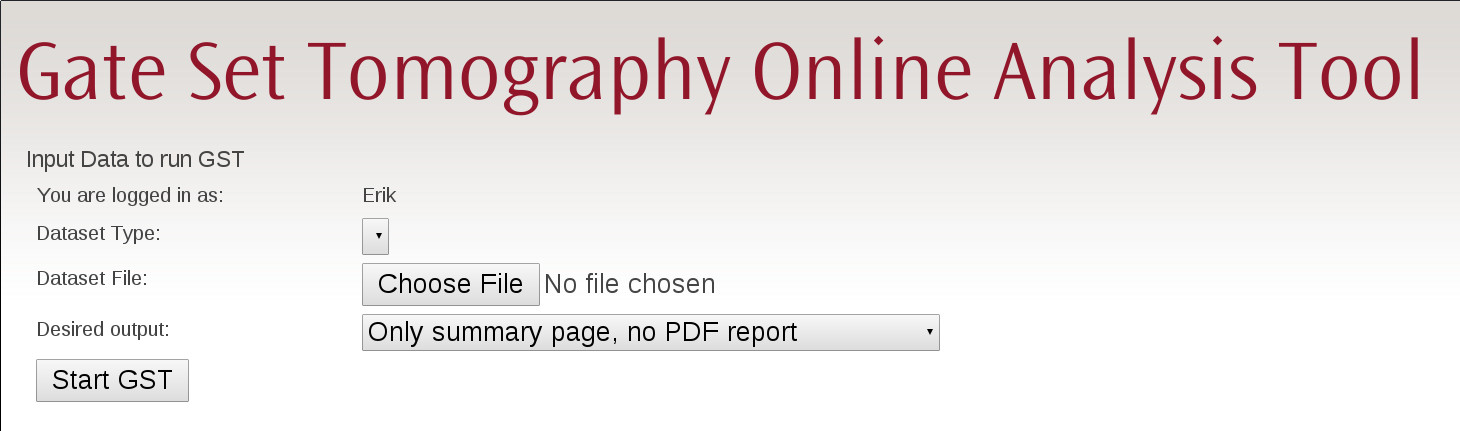
\includegraphics[width=6in]{QuickStartResources/StartPage.jpg}
\caption{GST Website Start Page\label{figStartPage}}
\end{center}
\end{figure}


\begin{enumerate}
\item Choose a dataset type: This tells GST what gates, fiducials, and germs, to use, as well as the maximum length of the strings you've used.  Thus, this tells GST what gate sequences to expect in the data file you upload.  Often times there's just one set of gates, fiducials, and germs that you're working with, and so selection of the dataset type amounts to selection of the maximum lengths you've used.  When we add dataset types for you, we often put this maximum length at the end of the dataset type name (e.g. the type \texttt{V1\_data\_512} has a maximum length of 512).
\item Choose a dataset file to upload: this one should be obvious.  Browse to the text-format file containing the data you want to analyze.  Note that this must be in GST's data file format.
\item Select whether you want GST to create a full blown PDF report (takes longer) or just show you a summary of the results in HTML tables without all the pretty figures that would be present in the full report.  Additionally, you can select whether to include appendices in the report, which makes the report generation take even longer.
\end{enumerate}

Once you've done these, just push the ``Start GST'' button, which brings you to the run page (Fig.~\ref{figRunPage}).  The run page contains a ``GST Status'' text box which shows you the output of GST as it runs.  It may take 10 seconds or so for this box to show anything, so please be patient.  If all goes well, GST will work its way through all its iterations and then display tables of the GST estimates beneath the status box (Fig.~\ref{figResultsPage}.  There will also be a link to the generated report if you selected that option.  

\begin{figure}
\begin{center}
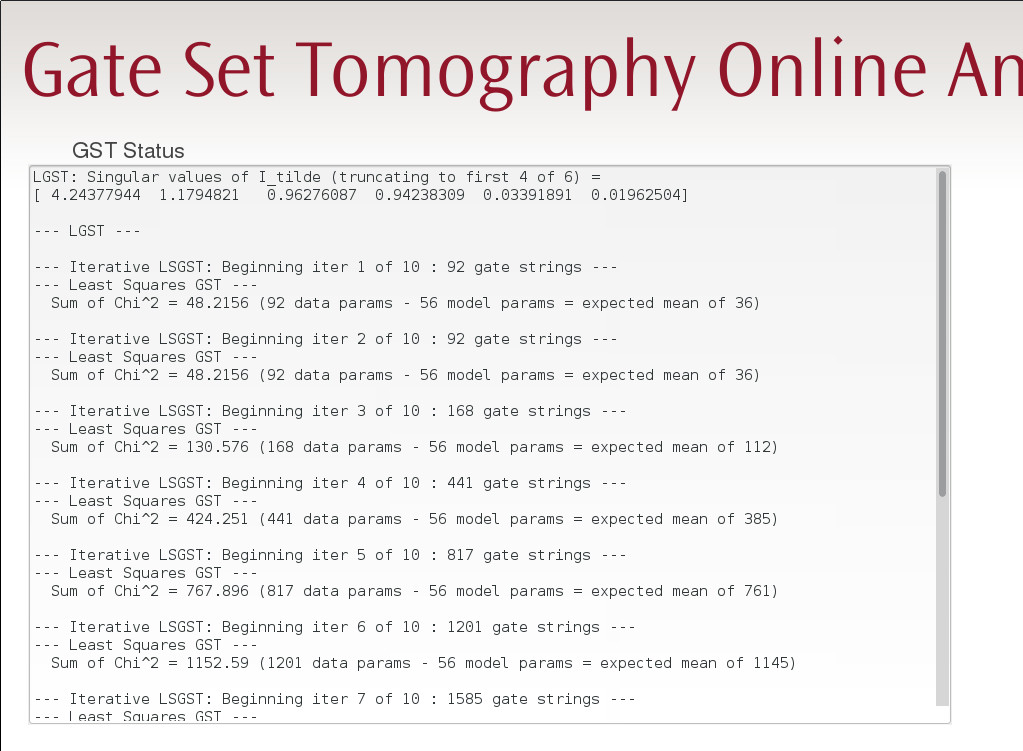
\includegraphics[width=6in]{QuickStartResources/StatusPage.jpg}
\caption{GST Website Run Page\label{figRunPage}}
\end{center}
\end{figure}


\begin{figure}
\begin{center}
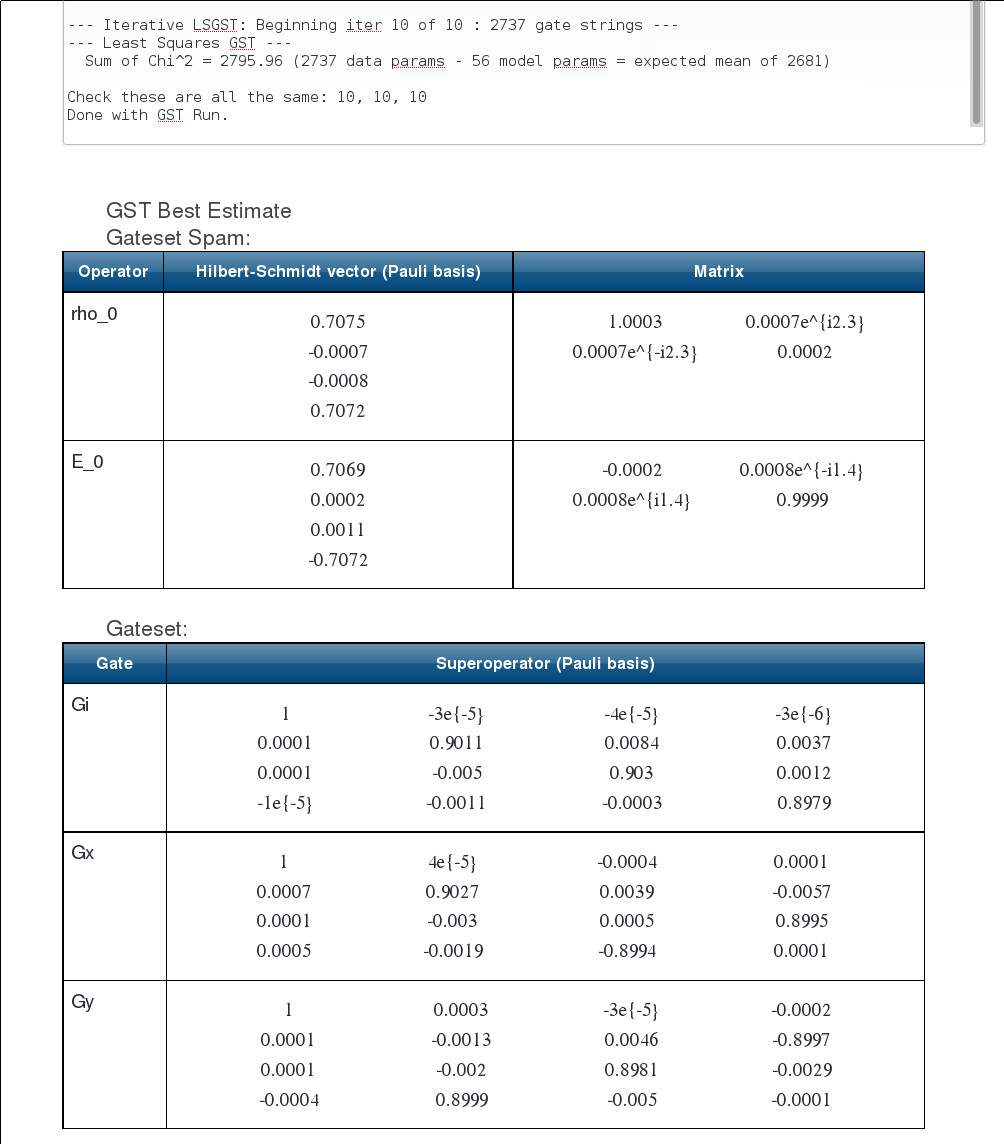
\includegraphics[width=6in]{QuickStartResources/ResultsPage.jpg}
\caption{GST Website Results Page\label{figResultsPage}}
\end{center}
\end{figure}


Finally, please note that the website is currently not a commercial-level web interface like Amazon.com, so try to be gentle.  For instance if you have multiple people from your group concurrently running GST things will break, so please coordinate.


\end{document}
